\chapter{Desenvolvimento de EVA}

\section{Apresentação do projeto}


A EVA (EV.G Virtual Assistant) é um \textit{chatbot} de domínio amplo que será capaz de interagir com os alunos vinculados ao EV.G na medida de suas necessidades.
Ela irá atender tais solicitações via mecanismo de conversação textual na plataforma de mensagens instantâneas chamada Telegram, no atendimento administrativo de uma secretaria acadêmica.

Por meio de EVA, os alunos vinculados ao EV.G poderão usufruir de várias funcionalidades.
Eles irão gerenciar seus cursos visualizando o andamento das inscrições, terão acesso ao catálogo unificado, calendário de turmas, histórico escolar e também serão auxiliados no processo de emissão de certificado. Tudo por meio de um acesso único e simplificado.

\section{Detalhamento dos requisitos de EVA}\label{especificacao-requisitos-eva}

Como dito \ref{cap:02:sec:05:projeto}, modelar o domínio de aplicação de um \textit{chatbot} é uma atividade de importante, pois, a partir desta atividade, pode se compreender a necessidade do sistema a ser construído, e também, definir os requisitos que o tornam útil.
É interessante deixar claro, que todo o processo de levantamento e validação dos requisitos foi realizado e entregue por parte da EV.G. Assim, não haverá nenhuma seção que aborde como se deu tal levantamento. Ao invés disso, os requisitos de EVA serão apenas detalhados nas subseções a seguir.

\subsection{Requisitos funcionais}

Na seção \ref{cap:02:sec:05:projeto:classificacao-requisitos}, foi explicado o que são os requisitos funcionais de um sistema. Abaixo, na Tabela \ref{tabela:tabela1}, estão listados os requisitos funcionais elencados para o sistema de EVA.

\begin{table}[htb]
\caption{Detalhamento de requisitos funcionais de EVA}
% \textsf{\caption{Especificação de requisitos funcionais de EVA}}
\label{tabela:tabela1}
% \center
% \footnotesize
\centering
\medskip
\begin{tabular}{|p{1.2cm}|p{3.5cm}|p{7.5cm}|}
  \hline
   \textbf{\#RF} & \textbf{Nome}  & \textbf{Descrição}  \\
    \hline
    RF01 & Conversação & Permitir que o usuário interaja com o \textit{chatbot} na língua portuguesa por meio de mensagens textuais em um \textit{messenger}. \\
    \hline
    RF02 & Compreensão & O \textit{chatbot} deve ser capaz de compreender o que o usuário solicita, através das mensagens textuais enviadas por ele, e tomar as devidas decisões para atende-lo. \\
    \hline
    RF03 & Autenticação & O \textit{chatbot} deve possuir uma forma de identificar o usuário que está solicitando acesso à aplicação. \\
   \hline
     RF04 & Visualizar o histórico escolar & O \textit{chatbot} deve informar ao usuário o seu histórico escolar completo caso seja solicitado por ele. \\
   \hline
    RF05 & Auxiliar na emissão de certificados & O \textit{chatbot} deve auxiliar o usuário no processo de emissão de certificados dos cursos concluídos por ele, caso seja solicitado por ele. \\
   \hline
    RF06 & Visualizar as inscrições de cursos abertos & O \textit{chatbot} deve exibir ao usuário quais inscrições de cursos que estão abertas, caso seja solicitado por ele. \\
   \hline
\end{tabular}
\end{table}

\subsection{Requisitos não funcionais}

Na seção \ref{cap:02:sec:05:projeto:classificacao-requisitos}, foi explicado o que são os requisitos não funcionais de um sistema. Abaixo, na Tabela \ref{tabela:tabela2}, estão listados os requisitos não funcionais elencados para o sistema de EVA.

\begin{table}[htb!]
\caption{Detalhamento de requisitos não funcionais de EVA}
\label{tabela:tabela2}
\center
\footnotesize
\begin{tabular}{|p{1.2cm}|p{3.5cm}|p{7.5cm}|}
  \hline
   \textbf{\#RNF} & \textbf{Nome}  & \textbf{Descrição}  \\
   \hline
    RNF01 & Disponibilidade & O sistema deve estar disponível continuamente (24 horas / 7 dias por semana). \\
   \hline
    RNF02 & Confidencialidade & O sistema deve garantir a visualização dos dados apenas pelo usuário associado. \\
   \hline
    RNF03 & Integridade & O sistema deve garantir que caso algum usuário falhe ao tentar se autenticar por três vezes consecutivas, bloqueie as tentativas de acesso dele durante 24 horas. \\
   \hline
   RNF04 & Portabilidade & O sistema deverá atender prioritariamente na plataforma de mensagens instantâneas Telegram. \\
   \hline
    RNF05 & Interoperabilidade & O sistema deverá se comunicar com algum serviço de Processamento de Linguagem Natural. \\
   \hline
    RNF06 & Implementação & O sistema deverá ser implementado utilizando a linguagem de programação Python. \\
   \hline
   
\end{tabular}
\end{table}\label{tabela:3}

\section{Casos de uso de EVA}

Na seção \ref{texto:especificando-com-casos-de-uso}, foi descrito o que são casos de uso e como eles normalmente são utilizados durante o projeto de um sistema. Elaborar os casos de uso permite definir quais funções de aplicação que o sistema deverá oferecer ao usuário~\cite{ReqJair}. Para a sua especificação, serão utilizados também alguns dos requisitos funcionais e não funcionais, que foram detalhados na seção \ref{especificacao-requisitos-eva}, para que se possa descrever as funcionalidades do sistema com ainda mais propriedade. Nas subseções a seguir, será realizado todo o processo de especificação e detalhamento dos casos de uso de EVA.

\subsection{Especificação dos atores}

Um ator é algo com comportamento, tal como uma pessoa (identificada por seu papel), um sistema ou uma organização~\cite{CraigLarman}. No que se diz respeito a EVA, foram identificados como atores o Visitante e o Aluno. Ambos poderão interagir com EVA, por meio de mensagens textuais, porém com as devidas restrições. É válido ressaltar, que a EVA não entra como ator, já que será o próprio sistema na qual está sendo modelando. Na Tabela \ref{tabela:tabela3} os atores são especificados.

\begin{table}[htb!]
\caption{Especificação dos atores do sistema de EVA}
\label{tabela:tabela3}
\center
\footnotesize
\begin{tabular}{|p{2cm}|p{3cm}|p{7.5cm}|}
  \hline
   \textbf{\#ATOR} & \textbf{Nome}  & \textbf{Descrição}  \\
   \hline
    ATOR01 & Visitante & Qualquer pessoa que interaja com EVA sem estar devidamente autenticado e identificado no sistema. \\
   \hline
    ATOR02 & Aluno & Qualquer pessoa que interaja com EVA e esteja devidamente autenticado e identificado no sistema. \\
   \hline
\end{tabular}
\end{table}


\subsection{Especificação dos casos de uso}

Como dito no começo desta seção, casos de uso permitem definir as funções de aplicação que o sistema deverá oferecer para o usuário. A partir dos requisitos funcionais identificados para EVA, foram extraídos os casos de uso especificados na Tabela \ref{tabela:tabela4}.
\begin{table}[htb!]
\caption{Especificação dos casos de uso de EVA}
\label{tabela:tabela4}
\center
\footnotesize
\begin{tabular}{|p{2cm}|p{3cm}|p{7.5cm}|}
  \hline
   \textbf{\#UC} & \textbf{Nome}  & \textbf{Descrição}  \\
   \hline
    UC01 & Dialogar com EVA & Os usuários do sistema poderão dialogar com EVA por meio de mensagens textuais, na língua portuguesa, através de um \textit{messenger}. A partir dessa funcionalidade, o usuário irá acessar todas as demais.\\
   \hline
    UC02 & Efetuar login & Autenticação de um usuário, permitindo que ele tenha acesso às funcionalidades restritas de EVA. \\
   \hline
    UC03 & Visualizar histórico escolar completo & O usuário poderá solicitar a visualização do histórico de todos os cursos que ele esteve matriculado no âmbito da EV.G. \\
   \hline
    UC04 & Receber auxílio na emissão de certificados & O usuário poderá solicitar auxilio para a emissão dos certificados dos cursos no qual ele finalizou no âmbito da EV.G. \\
   \hline
    UC05 & Visualizar inscrições de cursos abertos & O usuário poderá solicitar a visualização de todos os cursos na qual possui matricula ativa no âmbito da EV.G. \\
   \hline
    UC06 & Efetuar logout & O usuário deixará de estar autenticado no sistema. Com isso, ele volta a possuir acesso limitado às funcionalidades de EVA.\\
   \hline
\end{tabular}
\end{table}\label{tabela:3}

\subsection{Diagrama de casos de uso}

Para descrever de forma visual e clara como se dará o vínculo entre os atores e os casos de uso identificados de EVA, foi criado um diagrama de casos de uso. Para a criação deste, foi utilizada a notação UML.

Na UML, os atores são representados como figuras ‘palito’. Cada caso de uso, que são as possíveis interações que poderão ser realizadas, é representada por uma elipse. As linhas fazem a ligação entre os atores e as interações. Na Figura \ref{cap:03:fig:diagrama}, está representado o diagrama de casos de uso de EVA.
\begin{figure}
    \centering
    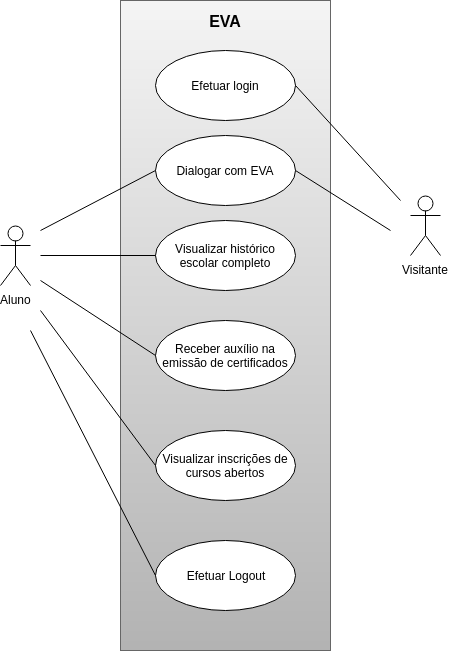
\includegraphics[width=0.7\linewidth]{src/imagens/CasoDeUsoEva.png}
    \caption{Fonte: Elaborado pelo autor (2018)}
    \label{cap:03:fig:diagrama}
\end{figure}

\subsection{Detalhamento dos casos de uso}

\subsubsection{UC01 - Dialogar com EVA}
\textbf{Descrição:} Este caso de uso especifica a ação principal de interação do usuário com o \textit{chatbot}, que é o diálogo. Por meio de mensagens textuais na língua portuguesa, o usuário poderá interagir com EVA e ter acesso à as suas funcionalidades. O nível de funcionalidades disponíveis para acesso do usuário, será determinada pelo fato dele estar autenticado ou não no sistema.

\begin{itemize}
    \item \textbf{Atores:}
        \begin{enumerate}
            \item ATOR01 - Visitante.
            \item ATOR02 - Aluno.
        \end{enumerate}
    \item \textbf{Requisitos funcionais:}
        \begin{enumerate}
            \item RF01 - Conversação.
            \item RF02 - Compreensão.
        \end{enumerate}
    \item \textbf{Requisitos não funcionais:}
        \begin{enumerate}
            \item RNF01 - Disponibilidade.
            \item RNF05 - Portabilidade.
            \item RNF05 - Interoperabilidade.
        \end{enumerate}
\end{itemize}

\textbf{Fluxo básico:} 
    \begin{enumerate}
        \item O usuário envia uma mensagem textual para EVA.
        \item EVA irá consultar sua base de conhecimento para compreender o que o ator solicita.
        \item EVA responde ao usuário com base no que foi compreendido.
    \end{enumerate}

\subsubsection{UC02 - Efetuar login}
\textbf{Descrição:} Este caso de uso especifica a ação de autenticação no sistema, com o objetivo de identificar o aluno vinculado ao EV.G, para que se possa auxilia-lo de maneira personalizada, tendo assim, acesso aos recursos mais sofisticados de EVA. O usuário irá informar o seu CPF ou e-mail, EVA irá consultar na sua base de dados afim de verificar se o usuário de fato possui um vinculo com a EV.G, e então será realizada a autenticação ou não.

\begin{itemize}
    \item \textbf{Atores:}
        \begin{enumerate}
            \item ATOR01 - Visitante.
            \item ATOR02 - Aluno.
        \end{enumerate}
    \item \textbf{Pré-condições:}
        \begin{enumerate}
            \item O usuário deve possuir um vinculo com a EV.G.
        \end{enumerate}
    \item \textbf{Pós-condições:}
        \begin{enumerate}
            \item O usuário terá acesso às funcionalidades mais personalizadas de EVA.
        \end{enumerate}
    \item \textbf{Requisitos funcionais:}
        \begin{enumerate}
            \item RF01 - Conversação.
            \item RF02 - Compreensão.
            \item RF03 - Autenticação.
        \end{enumerate}
    \item \textbf{Requisitos não funcionais:}
        \begin{enumerate}
            \item RNF01 - Disponibilidade.
            \item RNF02 - Confidencialidade.
            \item RNF03 - Integridade.
            \item RNF05 - Interoperabilidade.
        \end{enumerate}
\end{itemize}

\textbf{Fluxo básico:}
    \begin{enumerate}
        \item Ao início de uma conversação com EVA, ela irá solicitar que o usuário se identifique, para que ela possa lhe dar auxilio mais personalizado. Para isso, EVA irá solicitar que ele lhe informe o seu CPF ou e-mail cadastrados no EV.G.
        \item O usuário então irá informar o seu e-mail ou CPF.
        \item EVA irá verificar se o usuário está bloqueado no sistema.
        \item EVA irá verificar se o número de tentativas de autenticação chegaram ao valor limite, nesse caso, a três.
        \item EVA irá consultar em sua base de dados se as informações de fato conferem.
        \item O sistema então irá autenticar o usuário.
        \item EVA dá as boas vindas e informa ao usuário que a autenticação foi efetuada com sucesso.
        \item EVA apresenta as suas funcionalidades ao usuário e o convida a utilizar alguma.
    \end{enumerate}
    
\textbf{Fluxo alternativo A:}
    \begin{enumerate}
        \item No Passo 5 do Fluxo Básico, após EVA consultar sua base de dados, foi visto que as informações não conferem.
        \item A contagem para o limite de tentativas de autenticação de um usuário é incrementada em um.
        \item EVA então informa ao usuário que os dados não conferem e pede para que ele informe o CPF ou o e-mail novamente.
        \item O fluxo retornar ao Passo 2 do Fluxo básico.
    \end{enumerate}

\textbf{Fluxo alternativo B:}
    \begin{enumerate}
        \item No Passo 5 do Fluxo Básico, a mensagem texutal enviada pelo usuário não aparenta ser nem algo parecido com CPF ou e-mail.
        \item EVA informa que ao usuário que ele precisa informar o CPF ou o e-mail para que ele possa se identificar, e assim, para que eles possam continuar dialogando.
        \item O fluxo retorna ao Passo 2 do Fluxo básico.
    \end{enumerate}
    
\textbf{Fluxo alternativo C:}
    \begin{enumerate}
        \item No Passo 3 do Fluxo Básico, foi visto que o usuário está bloqueado no sistema.
        \item EVA informa que o usuário está bloqueado por um dia.
        \item EVA auxilia o usuário, que caso ele de fato ache que possui um vinculo com a EV.G, que ele entre em contato através do e-mail da EVG.
        \item EVA informa o e-mail.
        \item EVA pede desculpa pelo transtorno.
    \end{enumerate}
    
\textbf{Fluxo alternativo D:}
    \begin{enumerate}
        \item No Passo 4 do Fluxo Básico, foi visto que o usuário tentou se autenticar por três vezes sem sucesso.
        \item EVA bloqueia o usuário por um dia.
        \item EVA informa que o usuário está bloqueado por um dia.
        \item EVA auxilia o usuário, que caso ele de fato ache que possui um vinculo com a EV.G, que ele entre em contato através do e-mail da EVG.
        \item EVA informa o e-mail.
        \item EVA pede desculpa pelo transtorno.
    \end{enumerate}

\subsubsection{UC03 - Visualizar histórico escolar completo}
\textbf{Descrição:} Este caso de uso especifica a funcionalidade de EVA de pesquisar e informar o histórico escolar de um aluno vinculado ao EV.G. Para cada item identificado, EVA deve informar o nome do curso, a carga horária, o estado em que se encontra a matrícula do aluno e o estado de sua turma de ensino. 

\begin{itemize}
    \item \textbf{Atores:}
        \begin{enumerate}
            \item ATOR02 - Aluno.
        \end{enumerate}
    \item \textbf{Pré-condições:}
        \begin{enumerate}
            \item O usuário deve estar autenticado no sistema.
        \end{enumerate}
    \item \textbf{Requisitos funcionais:}
        \begin{enumerate}
            \item RF01 - Conversação.
            \item RF02 - Compreensão.
            \item RF04 - Visualizar histórico escolar.
        \end{enumerate}
    \item \textbf{Requisitos não funcionais:}
        \begin{enumerate}
            \item RNF01 - Disponibilidade.
            \item RNF02 - Confidencialidade.
            \item RNF04 - Portabilidade.
            \item RNF05 - Interoperabilidade.
        \end{enumerate}
\end{itemize}

\textbf{Fluxo básico:}
    \begin{enumerate}
        \item O aluno envia uma mensagem textual para EVA solicitando o seu histórico escolar.
        \item EVA irá consultar sua base de conhecimento para compreender o que o aluno solicita.
        \item EVA irá consultar a base de dados da EV.G para pesquisar os dados escolares do aluno.
        \item EVA irá formatar os dados encontrados para serem exibidos ao aluno.
        \item EVA irá informar ao alunos o seu histórico escolar completo. Para cada item identificado, EVA deverá especificar os nome do curso, a cargas horária, o estado da matrícula do aluno e o estado da turma de ensino.
    \end{enumerate}

\textbf{Fluxo alternativo A:}
    \begin{enumerate}
        \item No Passo 3 do Fluxo básico, foi constatado que o aluno não possui nenhuma matricula nos cursos da EV.G.
        \item EVA irá informar o aluno que ele não possui nenhuma matricula nos cursos da EV.G
        \item EVA irá sugerir ao aluno que ele visite o site da EV.G para ter acesso ao catálogo dos cursos oferecidos pela instituição.
    \end{enumerate}

\subsubsection{UC04 - Receber auxílio na emissão de certificados}
\textbf{Descrição:} Este caso de uso especifica a funcionalidade de EVA de auxiliar o aluno vinculado ao EV.G no processo de emissão de certificado. EVA irá pesquisar os cursos concluídos do aluno, e a partir destes, irá informar-lo quais procedimentos ele deverá realizar para emitir o certificado.

\begin{itemize}
    \item \textbf{Atores:}
        \begin{enumerate}
            \item ATOR02 - Aluno.
        \end{enumerate}
    \item \textbf{Pré-condições:}
        \begin{enumerate}
            \item O usuário deve estar autenticado no sistema.
        \end{enumerate}
    \item \textbf{Requisitos funcionais:}
        \begin{enumerate}
            \item RF01 - Conversação.
            \item RF02 - Compreensão.
            \item RF05 - Auxiliar na emissão de certificados.
        \end{enumerate}
    \item \textbf{Requisitos não funcionais:}
        \begin{enumerate}
            \item RNF01 - Disponibilidade.
            \item RNF02 - Confidencialidade.
            \item RNF04 - Portabilidade.
            \item RNF05 - Interoperabilidade.
        \end{enumerate}
\end{itemize}

\textbf{Fluxo básico:}

\textbf{Fluxo alternativo A:}

\subsubsection{UC05 - Visualizar inscrições de cursos abertos}
\textbf{Descrição:} Este caso de uso especifica a funcionalidade de EVA de pesquisar e informar quais inscrições de cursos de um aluno vinculado ao EV.G que estão em aberto. Para cada item identificado, EVA deve informar o nome do curso, a carga horária e o estado da turma. 

\begin{itemize}
    \item \textbf{Atores:}
        \begin{enumerate}
            \item ATOR02 - Aluno.
        \end{enumerate}
    \item \textbf{Pré-condições:}
        \begin{enumerate}
            \item O usuário deve estar autenticado no sistema.
        \end{enumerate}
    \item \textbf{Requisitos funcionais:}
        \begin{enumerate}
            \item RF01 - Conversação.
            \item RF02 - Compreensão.
            \item RF06 - Visualizar as inscrições de cursos abertos.
        \end{enumerate}
    \item \textbf{Requisitos não funcionais:}
        \begin{enumerate}
            \item RNF01 - Disponibilidade.
            \item RNF02 - Confidencialidade.
            \item RNF04 - Portabilidade.
            \item RNF05 - Interoperabilidade.
        \end{enumerate}
\end{itemize}

\textbf{Fluxo básico:}

\textbf{Fluxo alternativo A:}

\subsubsection{UC06 - Efetuar logout}
\textbf{Descrição:}

\begin{itemize}
    \item \textbf{Atores:}
        \begin{enumerate}
            \item ATOR02 - Aluno.
        \end{enumerate}
    \item \textbf{Pré-condições:}
        \begin{enumerate}
            \item O usuário deve estar autenticado no sistema.
        \end{enumerate}
    \item \textbf{Requisitos funcionais:}
        \begin{enumerate}
            \item RF01 - Conversação.
            \item RF02 - Compreensão.
        \end{enumerate}
    \item \textbf{Requisitos não funcionais:}
        \begin{enumerate}
            \item RNF01 - Disponibilidade.
            \item RNF02 - Confidencialidade.
            \item RNF04 - Portabilidade.
            \item RNF05 - Interoperabilidade.
        \end{enumerate}
\end{itemize}

\textbf{Fluxo básico:}


\section{Modelagem dos diálogos de EVA}

\subsection{Cenários}

\section{Arquitetura de EVA}

\subsection{Arquitetura da API}

\subsection{Arquitetura do \textit{chatbot}}